\documentclass[t,11pt]{beamer}

\usepackage[francais]{babel}
\usepackage[T1]{fontenc}
\usepackage[utf8]{inputenc}
\usepackage{hyperref}

\usetheme{Warsaw}
\setbeamercolor{background canvas}{bg=yellow!10!white}


\title{Introduction pragmatique à Git}
\author{K\'evin Unger\hspace{1mm} \newline kevin.unger@fresnel.fr}
\institute
{
        Institut Fresnel\\
        \url{https://github.com/kevung/git-presentation.git}
}
\date{\today}

\begin{document}

%----------------------------------------------
\begin{frame}[plain,c]
        \titlepage
\end{frame}

%----------------------------------------------
%table des matieres
\begin{frame}[c]
        \tableofcontents[hideallsubsections]
\end{frame}

%----------------------------------------------
%table des matieres auto a chaque section
\AtBeginSection[]{
\begin{frame}[c]
        \tableofcontents[currentsection,hideallsubsections]
\end{frame}
}

%----------------------------------------------
\section{Git?! A quoi ça sert\ldots}


\subsection{Situation n. 1}
\begin{frame}[label=sit1]
        \frametitle{Situation n. 1}
        \framesubtitle{Comment garder des traces sans perdre la tête?}
        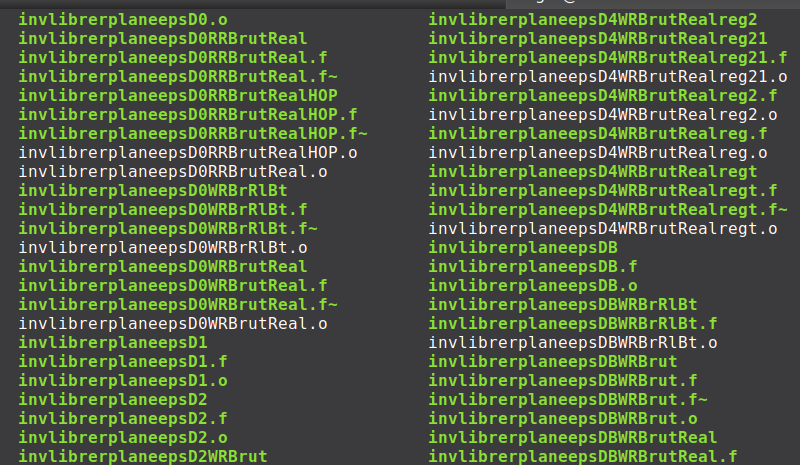
\includegraphics[width=\linewidth]{./img/bazar_crop2}
\end{frame}


\subsection{Situation n. 2}
\begin{frame}[label=sit2]
        \frametitle{Situation n. 2}
        \framesubtitle{Comment tester sans avoir peur de tout casser?}
\end{frame}


\subsection{Situation n. 3}
\begin{frame}[label=sit3]
        \frametitle{Situation n. 3}
        \framesubtitle{Comment travailler simultane\'ment sur un même document?}
\end{frame}

%----------------------------------------------
\section{Garder traces proprement}

\subsection{Principe}
\begin{frame}
        \frametitle{Principe}
        Principe du staging
\end{frame}

%----------------------------------------------
\section{Exp\'erimenter en toute s\'ecurit\'e}

\subsection{Principe}
\begin{frame}
        \frametitle{Principe}
        Principe du branching
\end{frame}

%----------------------------------------------
\section{Travailler \`a plusieurs (simultan\'ement) }

\subsection{Principe}
\begin{frame}
        \frametitle{Principe}
        Principe d'un d\'ep\^ot
\end{frame}

\end{document}
